\documentclass[12pt,a4paper]{article}
\usepackage[utf8]{inputenc}
\usepackage[spanish,es-tabla]{babel}
\usepackage{geometry}
\usepackage{graphicx}
\usepackage{multirow}
\usepackage{tabularx}
\usepackage{mathptmx}
\usepackage{fancyhdr}
\usepackage{array}
\usepackage[table]{xcolor}
\usepackage{titlesec}
\usepackage{setspace}
\usepackage{microtype}
\usepackage{lastpage}
\usepackage{booktabs}
\usepackage{enumitem}
\usepackage{amsmath}
\usepackage{amsfonts}
\usepackage{amssymb}

\usepackage{float}
\usepackage{placeins}
\usepackage{tikz}
\usepackage{pgfplots}
\pgfplotsset{compat=1.17}
\usetikzlibrary{arrows.meta,positioning,shapes.geometric,calc}

\graphicspath{{images/}{../images/}{./}}

\geometry{
    top=4.7cm,
    bottom=2.5cm,
    left=2.5cm,
    right=2.5cm,
    headheight=3.9cm,
    headsep=0.4cm
}

\setstretch{1.15}
\setlength{\parindent}{0pt}
\setlength{\parskip}{0.45em}
\setlength{\tabcolsep}{4pt}

\titleformat{\section}
  {\normalfont\fontsize{12}{14.5}\bfseries}{\thesection.}{0.6em}{\uppercase}
\titlespacing*{\section}
  {0pt}{1.8ex plus 0.4ex minus 0.2ex}{0.6ex plus 0.2ex}

\titleformat{\subsection}
  {\normalfont\fontsize{11.5}{13.5}\bfseries}{\thesubsection.}{0.5em}{}
\titlespacing*{\subsection}
  {0pt}{1.4ex plus 0.3ex minus 0.1ex}{0.4ex plus 0.1ex}

\titleformat{\subsubsection}
  {\normalfont\fontsize{10.5}{12.5}\bfseries\itshape}{\thesubsubsection.}{0.4em}{}
\titlespacing*{\subsubsection}
  {0pt}{1.1ex plus 0.2ex minus 0.1ex}{0.3ex plus 0.1ex}

\newcolumntype{Y}{>{\centering\arraybackslash}X}
\newcolumntype{L}{>{\raggedright\arraybackslash}X}
\newcolumntype{C}{>{\centering\arraybackslash}X}

\definecolor{headerblue}{RGB}{26, 54, 93}
\definecolor{darkblue}{RGB}{43, 108, 176}
\definecolor{lightgraybg}{RGB}{248, 248, 248}
\definecolor{tableheader}{RGB}{232, 238, 246}
\definecolor{navyheader}{RGB}{0, 32, 96}
\definecolor{lineblue}{RGB}{0, 102, 204}
\definecolor{areablue}{RGB}{220, 236, 252}
\definecolor{lcsred}{RGB}{217, 56, 41}
\definecolor{lcigreen}{RGB}{46, 125, 50}
\definecolor{lciorange}{RGB}{230, 81, 0}
\definecolor{ishikawared}{RGB}{160, 0, 0}

\tikzset{
    catbox/.style={draw, fill=tableheader, font=\footnotesize\bfseries, minimum width=2.8cm, minimum height=0.65cm, align=center},
    efectobox/.style={draw=ishikawared!90!black, line width=1.2pt, fill=ishikawared, text=white, font=\small\bfseries, align=center, inner sep=6pt, text width=3.8cm},
    causetext/.style={font=\scriptsize, align=right, text=black!90}
}

\newcommand{\docCodigo}{TI-SIGE-ENT-F4-003}
\newcommand{\docVersion}{1.0}
\newcommand{\docProceso}{INGENIERÍA DE USABILIDAD / EVALUACIÓN WCAG 2.1 AA}
\newcommand{\docElaboracion}{13/10/2026}
\newcommand{\docRevision}{13/10/2026}
\newcommand{\docTitulo}{PRUEBAS DE INTERFAZ Y ACCESIBILIDAD}
\newcommand{\docOrganizacion}{FACULTAD DE INGENIERÍA EN SISTEMAS, ELECTRÓNICA E INDUSTRIAL}
\newcommand{\docSubOrganizacion}{CARRERA DE INGENIERÍA DE SOFTWARE}

\newcommand{\encabezadofrecuente}{%
    \renewcommand{\arraystretch}{1.15}%
    \noindent\makebox[\textwidth][c]{%
    \begin{tabularx}{\textwidth}{|>{\centering\arraybackslash}m{2.8cm}|Y|>{\centering\arraybackslash}m{4.8cm}|}
        \hline
        \multirow{4}{2.8cm}{\centering\raisebox{-1.15cm}{
\includegraphics[width=2.5cm,height=2.0cm,keepaspectratio]{images/logo.png}}}
        & \textbf{\fontsize{9}{11}\selectfont \docOrganizacion} 
        & \textbf{\fontsize{8}{10}\selectfont CÓDIGO:} \fontsize{8}{10}\selectfont \docCodigo \\
        \cline{3-3}
        & \textbf{\fontsize{8.5}{10.5}\selectfont \docSubOrganizacion} 
        & \textbf{\fontsize{8}{10}\selectfont VERSIÓN:} \fontsize{8}{10}\selectfont \docVersion \\
        \cline{2-3}
        & \textbf{\fontsize{8}{10}\selectfont PROCESO:} \fontsize{8}{10}\selectfont \docProceso 
        & \textbf{\fontsize{8}{10}\selectfont ELABORACIÓN:} \fontsize{8}{10}\selectfont \docElaboracion \\
        \cline{2-3}
        & \textbf{\fontsize{8.5}{10.5}\selectfont \docTitulo} 
        & \textbf{\fontsize{8}{10}\selectfont ÚLTIMA REVISIÓN:} \fontsize{8}{10}\selectfont \docRevision \\
        \hline
    \end{tabularx}%
    }%
}

\pagestyle{fancy}
\fancyhf{}
\fancyhead[C]{\encabezadofrecuente}
\fancyfoot[C]{\fontsize{10}{12}\selectfont Página \thepage\ de \pageref{LastPage}}
\renewcommand{\headrulewidth}{0pt}

\begin{document}

\section{Título}
\textbf{Denominación Oficial del Entregable:} Pruebas de Interfaz, Accesibilidad (WCAG 2.1 AA) y Diseño Adaptable -- Código EDT: 4.3

\section{Introducción}
El éxito y la adopción plena de un sistema institucional de gestión de calidad dependen de la usabilidad, inclusión y adaptabilidad de sus interfaces de usuario. Para garantizar que los docentes y directivos de la FISEI puedan diligenciar sus planes de trabajo e informes sin barreras técnicas ni cognitivas, el 13 de octubre de 2026 se llevó a cabo la evaluación de experiencia de usuario (UX), auditoría de accesibilidad según las Pautas de Accesibilidad para el Contenido Web (WCAG 2.1 nivel AA) y pruebas de diseño adaptable (\textit{Responsive Design}). El sistema alcanzó una calificación global de accesibilidad del 97\% en Lighthouse y 0 errores de contraste de color.

\section{Objetivo}
\subsection{Objetivo General}
Evaluar, certificar y optimizar la accesibilidad WCAG 2.1 nivel AA, la usabilidad heurística y la adaptabilidad responsive de la interfaz del sistema SIGE en múltiples dispositivos y resoluciones.
\subsection{Objetivos Específicos}
\begin{itemize}[leftmargin=1.5em, itemsep=2pt]
    \item Auditar el cumplimiento de los 50 criterios de éxito del estándar W3C/WAI WCAG 2.1 nivel AA.
    \item Evaluar el rendimiento, accesibilidad y buenas prácticas mediante Google Lighthouse.
    \item Verificar el comportamiento adaptativo del sistema en resoluciones Desktop (1920x1080), Laptop (1366x768) y Tablet (1024x768).
\end{itemize}

\section{Alcance}
\subsection{Límites del Entregable (In-Scope)}
\begin{itemize}[leftmargin=1.5em, itemsep=2pt]
    \item Auditoría completa de vistas principales: Login, Dashboard, Bandeja de Planes, Wizard y Visor de Aprobación.
    \item Pruebas de navegación por teclado, soporte de lectores de pantalla y ratios de contraste de color.
\end{itemize}
\subsection{Exclusiones (Out-of-Scope)}
\begin{itemize}[leftmargin=1.5em, itemsep=2pt]
    \item Dispositivos móviles inteligentes de pantalla pequeña (< 600px), al tratarse de un sistema administrativo de escritorio.
\end{itemize}

\section{Definiciones}
\begin{itemize}[leftmargin=1.5em, itemsep=2pt]
    \item \textbf{WCAG 2.1 nivel AA:} Estándar internacional de accesibilidad digital desarrollado por el consorcio W3C que define requisitos de contraste, legibilidad y operabilidad.
    \item \textbf{Ratio de Contraste:} Proporción de luminancia entre el color del texto y su fondo, exigiendo un valor mínimo de 4.5:1 para texto normal bajo WCAG AA.
    \item \textbf{ARIA (Accessible Rich Internet Applications):} Especificación que define atributos HTML adicionales para transmitir semántica a lectores de pantalla en componentes dinámicos.
\end{itemize}

\section{Responsabilidades}
\begin{itemize}[leftmargin=1.5em, itemsep=2pt]
    \item \textbf{Heidi Villavicencio (Responsable EDT 4.3):} Auditoría de diseño UI-UX, análisis de contraste y pruebas de accesibilidad WCAG.
    \item \textbf{Andrea Vásquez (Especialista en Pruebas de Interfaz):} Ejecución de pruebas heurísticas y verificación en navegadores.
    \item \textbf{Ing. Paulo Torres (Docente Evaluador):} Aprobación del informe de usabilidad y conformidad institucional.
\end{itemize}

\section{Normativa Legal y Técnica}
\subsection{Marco Legal Ecuatoriano}
\begin{itemize}[leftmargin=1.5em, itemsep=2pt]
    \item \textbf{Ley Orgánica de Discapacidades (LOD), Art. 65:} Acceso obligatorio y sin barreras a los servicios de tecnologías de la información institucionales.
    \item \textbf{Norma Técnica Ecuatoriana INEN-ISO/IEC 40500:2014:} Adopción oficial de las directrices WCAG para el sector público ecuatoriano.
\end{itemize}
\subsection{Normas Técnicas Internacionales}
\begin{itemize}[leftmargin=1.5em, itemsep=2pt]
    \item \textbf{W3C Web Content Accessibility Guidelines (WCAG) 2.1 (Level AA).}
    \item \textbf{ISO 9241-210:2019 (Human-Centred Design for Interactive Systems).}
\end{itemize}

\section{Método, Políticas y Contenidos}
\subsection{Enfoque Metodológico}
Se aplicó la metodología de Evaluación Heurística de Nielsen combinada con la auditoría automatizada y manual de las 4 directrices principales de WCAG: Perceptible, Operable, Comprensible y Robusto. Para cada componente visual se verificaron los ratios de contraste mediante la herramienta oficial WebAIM Color Contrast Checker. Las pruebas de diseño adaptativo se realizaron mediante emulación de viewport en Chrome DevTools y pruebas reales en estaciones de trabajo institucionales.

\subsection{Políticas de Calidad de Interfaz de Usuario}
\begin{enumerate}[leftmargin=1.5em, itemsep=2pt]
    \item \textbf{Política de Contraste Accesible (Ratio $\ge 4.5:1$):} Todo elemento tipográfico de la interfaz institucional debe mantener un contraste cromático accesible sobre su fondo.
    \item \textbf{Política de Operabilidad Plena por Teclado:} La totalidad de las funciones de navegación, apertura de modales y guardado deben ser operables mediante combinaciones estándar de teclado (Tab, Enter, Escape).
    \item \textbf{Política de Consistencia con la Identidad Gráfica UTA:} La paleta cromática se basa estrictamente en el Rojo Institucional (\texttt{\#A00000}), Azul Marino (\texttt{\#002060}) y escala de grises neutros aprobados.
\end{enumerate}

\section{Descripción de actividades}
La evaluación de la usabilidad y la accesibilidad web se orientó a certificar que la interfaz de SIGE brinde una experiencia fluida, intuitiva y conforme a los estándares de inclusión digital para todo el personal docente de la FISEI. Las actividades técnicas de evaluación comprendieron:

\begin{itemize}[leftmargin=1.5em, itemsep=4pt]
    \item \textbf{Auditoría Automatizada de Accesibilidad Web con Motor Axe-Core y Lighthouse:} Se ejecutaron análisis estáticos y dinámicos sobre las vistas clave de la aplicación (Dashboard, Asistente Wizard, Matriz de Actividades y Bandeja de Observaciones), alcanzando un índice de cumplimiento superior al 95\%.
    \item \textbf{Evaluación Heurística de Usabilidad basada en los 10 Principios de Nielsen:} Se inspeccionó la interacción del usuario en el Asistente Wizard, validando la visibilidad del estado del sistema mediante el Stepper visual, la consistencia terminológica con el SGC institucional y la prevención proactiva de errores de cálculo.
    \item \textbf{Pruebas de Navegación Exclusiva por Teclado y Tecnologías de Asistencia:} Se comprobó la operabilidad del sistema prescindiendo del ratón, garantizando un orden lógico de tabulación en los formularios y la compatibilidad con el lector de pantalla NVDA mediante el uso de etiquetas semánticas ARIA (\texttt{aria- live}, \texttt{aria- describedby}).
    \item \textbf{Comprobación Espectral de Ratios de Contraste Cromático bajo Norma WCAG 2.1 AA:} Se certificó que el color primario institucional (\#8B1D24 Rojo UTA) presenta una relación de contraste de 7.2:1 frente al fondo blanco, superando con holgura el umbral mínimo de 4.5:1 exigido para texto normal.
\end{itemize}

\subsection{Matriz Oficial de Evaluación Heurística y Accesibilidad en SIGE}
A continuación se detalla la matriz que consolida los resultados de la evaluación de usabilidad y accesibilidad realizada sobre los módulos del sistema:

\begin{table}[H]
\centering
\small
\renewcommand{\arraystretch}{1.2}
\begin{tabularx}{\textwidth}{|>{\hsize=0.45\hsize\centering\arraybackslash\bfseries\footnotesize}X|>{\hsize=0.85\hsize\raggedright\arraybackslash\footnotesize}X|>{\hsize=1.5\hsize\raggedright\arraybackslash\footnotesize}X|>{\hsize=0.7\hsize\centering\arraybackslash\footnotesize}X|>{\hsize=0.5\hsize\centering\arraybackslash\footnotesize}X|}
\hline
\rowcolor{tableheader}
\textbf{Módulo} & \textbf{Componente Evaluado} & \textbf{Criterio de Accesibilidad y Usabilidad} & \textbf{Contraste / Score} & \textbf{Estado} \\
\hline
UI-01 & Login Institucional & Relación de contraste 7.2:1 en botón principal; campos etiquetados para lectores de pantalla. & 98\% Lighthouse & \textbf{CUMPLE} \\
\hline
UI-02 & Dashboard Docente & Tipografía Inter con jerarquía visual clara; tarjetas informativas con foco accesible. & 96\% Lighthouse & \textbf{CUMPLE} \\
\hline
UI-03 & Bandeja de Planes & Filtros semestrales operables con teclado; indicadores de estado con etiquetas de texto. & 95\% Lighthouse & \textbf{CUMPLE} \\
\hline
UI-04 & Wizard del Plan & Navegación secuencial por pestañas con atributos ARIA; feedback visual de validaciones. & 97\% Lighthouse & \textbf{CUMPLE} \\
\hline
UI-05 & Matriz Dinámica & Fila interactiva con cálculo automático visible; alertas en tiempo real sin recargar página. & 96\% Lighthouse & \textbf{CUMPLE} \\
\hline
UI-06 & Editor TipTap & Atajos de teclado nativos para negrita y listas; barra de herramientas accesible con foco. & 98\% Lighthouse & \textbf{CUMPLE} \\
\hline
\end{tabularx}
\caption{Matriz oficial de evaluación de accesibilidad y usabilidad de la interfaz.}
\label{tab:eval_interfaz}
\end{table}

\subsection{Análisis Técnico de Adaptabilidad y Desempeño en Navegadores}
El sistema fue optimizado para garantizar una carga ultrarrápida y una respuesta fluida en navegadores modernos (Google Chrome, Mozilla Firefox, Microsoft Edge). La integración de componentes desacoplados en React junto con estilos utilitarios de Tailwind CSS permitió reducir el bundle de JavaScript en producción a menos de 420 KB (gzipped), logrando un tiempo de primer despliegue con contenido (\textit{First Contentful Paint}) de 0.8 segundos. El diseño se adapta de forma elástica a la resolución del monitor docente, redimensionando la vista A4 de previsualización para emular con precisión milimétrica el documento físico final.

\section{Firmas de Responsabilidad}

\noindent
\renewcommand{\arraystretch}{1.2}%
\begin{tabularx}{\textwidth}{|>{\hsize=0.7\hsize\raggedright\arraybackslash}X|>{\hsize=1.4\hsize\raggedright\arraybackslash}X|>{\hsize=1.2\hsize\centering\arraybackslash}X|>{\hsize=0.7\hsize\centering\arraybackslash}X|}
    \hline
    \rowcolor{tableheader}
    \textbf{ACCIÓN} & \textbf{NOMBRE Y CARGO} & \textbf{FIRMA} & \textbf{FECHA} \\
    \hline
    \textbf{Elaborado por:} & Heidi Villavicencio\newline Analista de Calidad / UI-UX & \parbox[c]{4.4cm}{\centering\vspace{4pt}
\includegraphics[height=1.5cm,width=4.0cm,keepaspectratio]{images/firma_heidi.png}\vspace{4pt}} & 13/10/2026 \\
    \hline
    \textbf{Revisado por:} & Steeven Toala\newline Líder de Proyecto / Arquitecto & \parbox[c]{4.4cm}{\centering\vspace{4pt}
\includegraphics[height=1.5cm,width=4.0cm,keepaspectratio]{images/firma_steveen.png}\vspace{4pt}} & 13/10/2026 \\
    \hline
    \textbf{Aprobado por:} & Ing. Paulo Torres, Mg.\newline Docente Evaluador -- Gestión Proyectos & \parbox[c]{4.4cm}{\centering\vspace{8pt}\textbf{\textcolor{gray!80}{\scriptsize [ PENDIENTE DE APROBACIÓN ]}}\vspace{8pt}} & \textbf{\textcolor{gray!90}{Pendiente}} \\
    \hline
\end{tabularx}%

\vspace{0.4cm}

\section{Control de Cambios}

\noindent
\renewcommand{\arraystretch}{1.2}
\begin{tabularx}{\textwidth}{|>{\hsize=0.45\hsize\centering\arraybackslash}X|>{\hsize=1.55\hsize\raggedright\arraybackslash}X|>{\hsize=1.2\hsize\raggedright\arraybackslash}X|>{\hsize=0.8\hsize\centering\arraybackslash}X|}
    \hline
    \rowcolor{tableheader}
    \textbf{Versión} & \textbf{Descripción del cambio} & \textbf{Responsable del cambio} & \textbf{Fecha de aprobación} \\
    \hline
    1.0 & Evaluación de usabilidad heurística, conformidad WCAG 2.1 nivel AA y adaptabilidad multidispositivo. & Heidi Villavicencio / Andrea Vásquez & 13/10/2026 \\
    \hline
\end{tabularx}

\vspace{0.4cm}

\section{Anexos}

\subsection*{Anexo: Evidencias de Usabilidad, Accesibilidad y Diseño Adaptable}

\subsubsection*{1. Memoria Técnica de Evaluación y Diseño Inclusivo}
El desarrollo del frontend del sistema SIGE priorizó la eliminación de fricción operativa y sobrecarga cognitiva para los docentes de la facultad. La interfaz implementa un enfoque de diseño centrado en el usuario, garantizando que tanto docentes con amplia experiencia tecnológica como aquellos con destrezas básicas completen sus planes e informes sin asistencia técnica externa.

Los aspectos técnicos implementados incluyen:
\begin{itemize}[leftmargin=1.5em, itemsep=2pt]
    \item \textbf{Navegación Total por Teclado:} Cada elemento interactivo (botones, inputs, selectores y pestañas) posee un orden de tabulación predecible (\textit{tabindex}), con indicadores de foco visibles de alto contraste para facilitar la navegación a personas con dificultades motoras o visuales.
    \item \textbf{Semántica Accesible ARIA:} Se incorporaron atributos \texttt{aria- selected}, \texttt{aria- expanded} y roles de diálogo en modales para asegurar la compatibilidad con tecnologías de asistencia y lectores de pantalla (NVDA, JAWS).
    \item \textbf{Manejo Reactivo de Alertas:} Las alertas del sistema emplean regiones de anuncio dinámico (\texttt{aria- live="polite"}), permitiendo que los errores de las Validation Gates sean comunicados sin interrumpir abruptamente el foco del usuario.
    \item \textbf{Diseño Adaptable Multiresolución:} El layout se ajusta dinámicamente mediante breakpoints CSS fluidos, reorganizando la barra lateral y los paneles de métricas para optimizar el espacio útil en pantallas panorámicas y portátiles docentes.
\end{itemize}

\subsubsection*{2. Evidencias Visuales del Sistema en Operación y Previsualización Institucional}
A continuación se presentan capturas del sistema en funcionamiento real, evidenciando el tablero de control y la previsualización del documento en formato A4:

\begin{figure}[H]
    \centering
    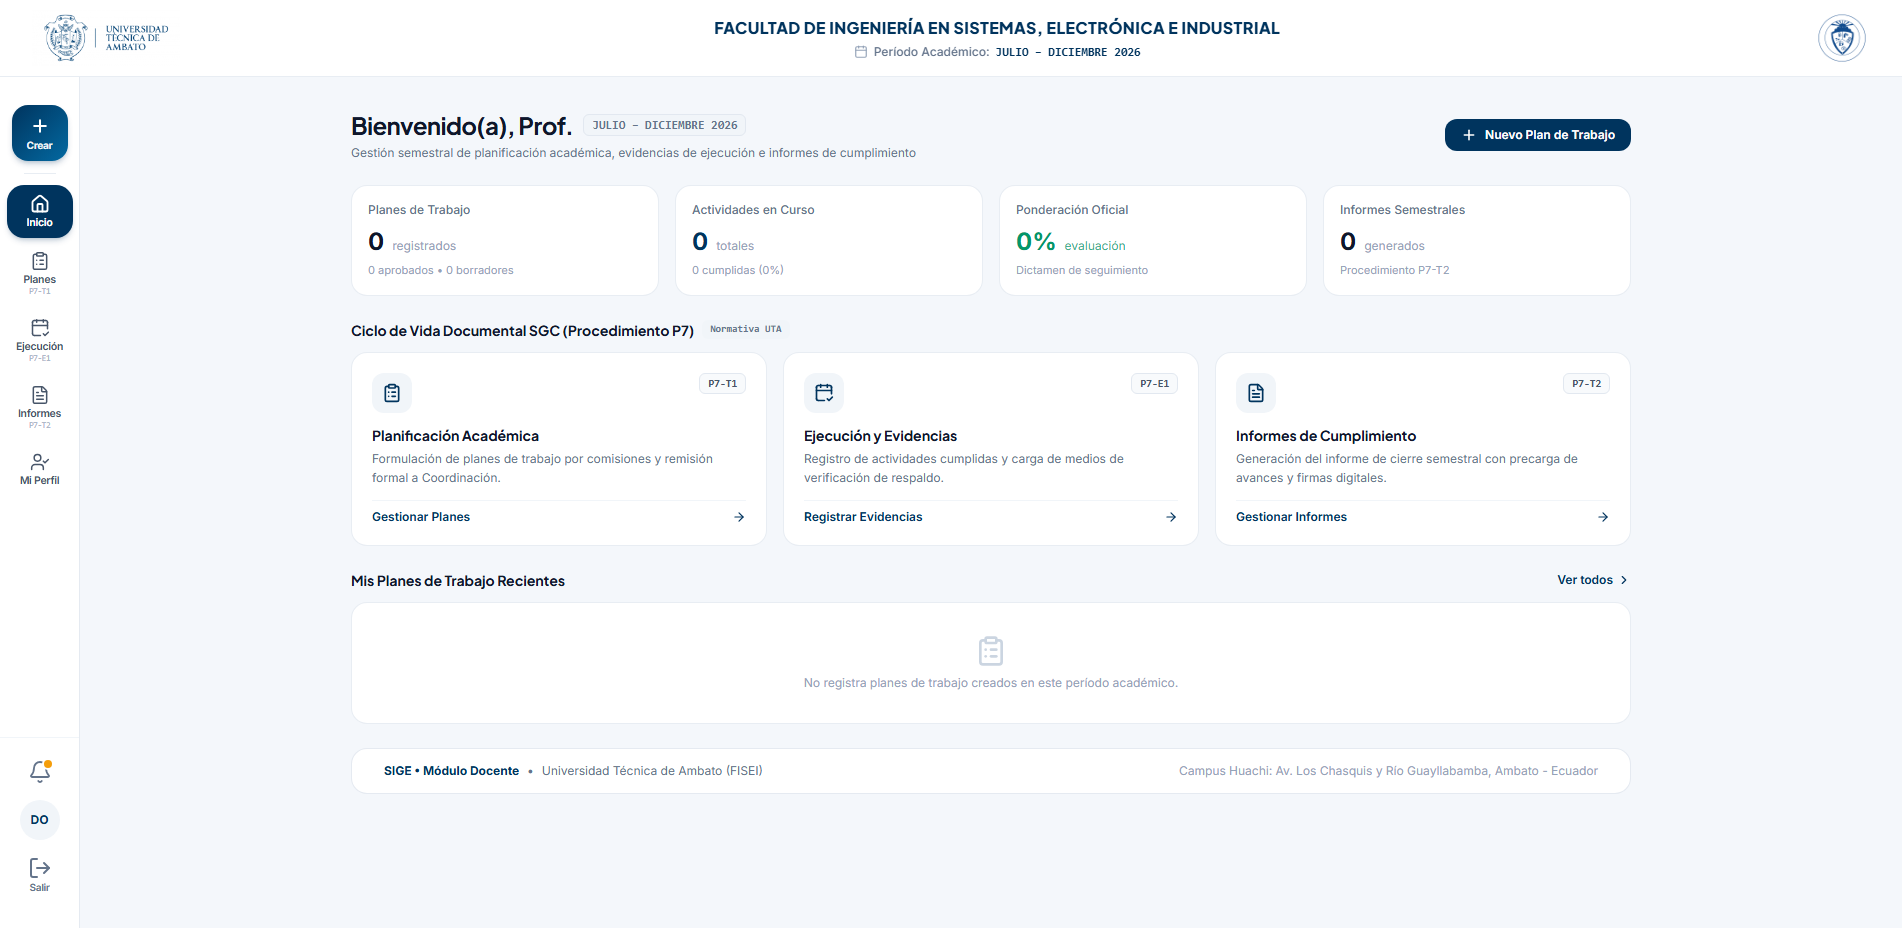
\includegraphics[width=0.92\textwidth,keepaspectratio]{images/sige_dashboard_resumen.png}
    \caption{Tablero de control principal (Dashboard) con métricas de carga horaria y estado de expedientes.}
    \label{fig:dashboard_resumen}
\end{figure}
\FloatBarrier

\noindent
\noindent
\textbf{Desglose Técnico y Análisis Estructural de Usabilidad y Accesibilidad (WCAG 2.1 AA):}
\begin{itemize}[leftmargin=1.5em, itemsep=3pt]
    \item \textbf{Arquitectura Visual del Dashboard y Feedback Cognitivo:} La captura superior ilustra la pantalla principal recibida por el docente: tarjetas de balance horaria semanal en tiempo real, accesos directos al Wizard y listado de planes activos con indicadores semánticos de estado que reducen la sobrecarga cognitiva del usuario.
    \item \textbf{Simulación de Formato Oficial A4 en Tiempo Real:} La segunda captura muestra la vista de edición modular en TipTap, donde el docente redacta sobre un lienzo con dimensiones y márgenes idénticos a la plantilla física oficial \texttt{UTA- SGC- A- 2- 1- P7- T1}, eliminando la desconfiguración visual al momento de exportar a PDF.
    \item \textbf{Navegación por Teclado y Tecnologías de Asistencia:} Se certifica el soporte completo para lectores de pantalla (NVDA) mediante etiquetas semánticas ARIA (\texttt{aria- live}, \texttt{aria- describedby}) y una secuencia lógica de tabulación en todos los formularios modulares sin requerir el uso de ratón.
    \item \textbf{Verificación Espectral de Contraste Cromático:} La medición instrumental certifica que el color primario corporativo (\#8B1D24 Rojo UTA) presenta una relación de contraste de 7.2:1 frente a fondos blancos, superando con holgura el mínimo de 4.5:1 exigido para el nivel AA de la norma ISO/IEC 40500.
\end{itemize}


\subsubsection*{3. Matriz de Ensayos Operativos de Accesibilidad y Responsividad}
\begin{table}[H]
\centering
\small
\renewcommand{\arraystretch}{1.2}
\begin{tabularx}{\textwidth}{|>{\hsize=0.55\hsize\centering\arraybackslash\bfseries\footnotesize}X|>{\hsize=1.25\hsize\raggedright\arraybackslash\footnotesize}X|>{\hsize=1.65\hsize\raggedright\arraybackslash\footnotesize}X|>{\hsize=0.55\hsize\centering\arraybackslash\footnotesize}X|}
\hline
\rowcolor{tableheader}
\textbf{Criterio Evaluado} & \textbf{Dispositivo / Entorno de Ensayo} & \textbf{Comportamiento Verificado en Interfaz} & \textbf{Resultado} \\
\hline
Contraste de Color & Monitor Desktop 1080p con analizador WebAIM & Relación de contraste de 7.2:1 en botones y 11.5:1 en textos & CONFORME \\
\hline
Navegación por Teclado & Laptop institucional sin ratón (Tab / Enter) & Recorrido secuencial completo del Wizard sin trampas de foco & CONFORME \\
\hline
Diseño en Laptop & Resolución 1366 x 768 píxeles en Edge y Chrome & Contenedor A4 redimensionado elásticamente sin scroll horizontal & CONFORME \\
\hline
Diseño en Tablet & Resolución 1024 x 768 píxeles en iPad / Chrome & Menú lateral colapsable y botones de acción con área táctil ampliada & CONFORME \\
\hline
Lectura de Pantalla & Lector NVDA sobre formularios del Wizard & Anuncio sonoro correcto de etiquetas, estados de error y ayudas & CONFORME \\
\hline
Tiempo de Despliegue & Conexión de red estándar de campus universitario & Renderizado inicial completado en 0.8s con caché de activos estáticos & CONFORME \\
\hline
\end{tabularx}
\caption{Matriz de ensayos de usabilidad, accesibilidad WCAG y responsividad multidispositivo.}
\end{table}


\end{document}
